\documentclass[11pt]{article}
\usepackage[margin=1in]{geometry}
\usepackage{mathabx}
\usepackage{multicol}
\usepackage{graphicx}

\begin{document}



\title{Epitaxial growth of samarium nitride on yttria stabilized zirconia}
\author{William Holmes-Hewett under the supervision of Joe Trodahl and Ben Ruck}
\maketitle




\twocolumn
\sloppy

\section{Introduction}
The rare earth elements form he section of the periodic table over which the $4f$ electron shell is filled. This gives them interesting magnetic properties which vary widely over the series. $Sm$ and $Gd$ are of express interest due to their electronic configurations. Both take the form $4f_x5d_26s_1$ where $Sm$ has 5 $4f$ electrons and $Gd$ has 7. When grown as rear earth nitrides both of these elements form the $NaCl$ rock-salt structure giving up their $5d$ and $6s$ electrons to nitrogen atoms. Leaving the electronic configuration in the case of samarium nitride of $4f_5$ and gadolinium nitride as $4f7$.

By applying Hund's rules to these configurations we see that $GdN$ will have a magnetization of $7\mu_B$ per $Gd$ and $SmN$ will have a vanishingly small net magnetization due to cancellation between orbital and spin magnetic moments. In perfectly stoichiometric samples both $GdN$ and $SmN$ are insulators with all conduction electrons used to create nitrogen bonds, however any nitrogen vacancy $(N_v)$ in the lattice can contribute up to three conduction electrons to the material, thus the carrier concentration may be doped by altering the amount of $N_v$. These properties include $SmN$ and $GdN$ to the small class of magnetic semiconductors, making them of interest to the area of spintronics. Of even more interest is that doping either material with $N_v$ will not influence  its magnetic properties, making these materials somewhat unique. Not only is $SmN$ the only known near net zero ferromagnetic semiconductor [reference] but it has also displayed superconductivity when heavily doped with $N_v$ while in its ferromagnetic phase.

The electronic structure of $GdN$ has been the subject of several studies [reference] and its band structure is mostly understood [check this]. The band structure of $SmN$ however is much less understood, particularity the band gap in the ferromagnetic phase [check this] and the location of the lowest $4f$ level in the conduction band. If a clearer picture of the band structure of $SmN$ were provided some of its more interesting and unique properties may be able to be understood.

One measurement technique that may provide information on the band structure of $SmN$ is angle resolved photo-electron spectroscopy (ARPES). ARPES measures both the speed and scattering of electrons excited out of a sample by soft x-rays. This enables the determination of both the energy and momentum enabling the band structure to be reconstructed. As only electrons excited from a sample are measured ARPES only yields information regarding the density of states in the valence band of a given material. 
ARPES measurements on $SmN$ may provide new information into the band structure and although only the conduction band would be probed these measurements are of obvious value. For ARPES measurements to be successful a sample must be single crystal and as close as possible to atomically flat, this is as the angle of emission of excited electrons from the sample must be determined. The manufacture of these samples was the primary goal of this project. 
\begin{figure}[b!]


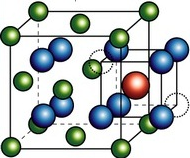
\includegraphics[width=\linewidth]{YSZ_Wikipedia.png}
\label{fig:boat1}
\caption{YSZ displays a cubic face on [100] and a lattice parameter that matches very well with RENs, however mobile $O^-$ ions due to vacanies can cause an oxide layer to form at the sample substrate interface.}
\end{figure}


Previous work has been completed regarding the epitaxial growth of $SmN$[big one and jay]. Chan et al. report on the occurrence of multiple rotational domains in epitaxial $SmN$ grown on a hexagonal $AlN$ net, while Natalie et. al. report on the lattice mismatches between possible substrates and the REN series. It is desirable to grow a single crystal sample with a minimal lattice mismatch to reduce strain. This requires a cubic net with a similar lattice parameter to $SmN$, such requirements can be found in Yttriua stabilized zirconiua (YSZ) which on its [100] face has a cubic net with and a lattice parameter of $5.12\mathring{A}$ a $98$ match to $SmN$ which has a lattice parameter of $5.02\mathring{A}$.


The cubic net of [100] YSZ along with the small lattice mismatch with $SmN$ may make it look very appealing for single crystal epitaxial growth, however a diligent experimentalist will soon notice a caveat. The crystal structure of YSZ pictured in figure [???] displays an $O^-$ vacancy, this makes YSZ an efficient $O^-$ ionic conductor which finds important application in fuel cell technology, however causes problems in teh fabrication of RENs. RENs have a proficiency to degrade to their oxide form $Re_2O_3$ when exposed to oxygen [source]. This is normally mitigated by the use of a capping layer, typically $AlN, GaN$ or metallic $Sm$ or $Gd$. This capping layer can not however protect a sample from its own substrate. Thus it is expected an oxide layer would form at the interface between a sample and its substrate, this
was observed by Ludbrook et al. [ref] in similar growths involving $GdN$ Thus for the creation of a successful sample the the mobile $O^-$ ions must be removed from the YSZ substrate. The thermal emission characteristics of $O^-$ ions from YSZ is shown by Fujiwara et. al. [ref] to follow an exponential relationship as would be naively expected from the Boltzmann equation. 

\section{Experimental Methods}

Before samples were grown experiments were carried out on bare YSZ substrates to determine if it was possible to deplete the levels of $O^-$ ions enough to avoid the creation of an oxide layer at the sample-substrate interface. This involved baking the substrate at temperatures well above the growth temperature while monitoring the gas composition inside the chamber using a mass spectrometer. Initial tests indicated that it may be possible to measurably deplete the mobile ions. Figure [] shows the amount of oxygen in the chamber as a function of time, which can be clearly seen to increase with temperature and drop once a stable temperature has been reached. The sample was then taken to growth temperature until a stable oxygen level was achieved, the temperature was then raised well above the growth temperature for several hours, following this the sample was taken back to the growth temperature where a lower concentration of oxygen could be observed than previous.

 
Samples were grown on 10mm x 10mm x 0.5mm YSZ [100] substrates, which were back for various times before growth from 2  to 8 hours. Growth temperatures were $600^\degree$C under an atmosphere of $1e^{-4}$mb of 99.999\% pure nitrogen with a $Sm$ flux of $1-5\mathring{A}/s$. Nitrogen was not ionized, instead the catalytic cracking of $N_2$ molecules on contact with rare earths was used. During growth the sample surface was monitored using reflection high energy electron diffraction (RHEED) this enabled the \emph{insitu} measurement of the evolution of the lattice parameter. To prevent oxidation of the surface layer sample were capped with either $Sm$ metal or $AlN$. Following growth X-ray diffraction (XRD) measurements were taken to confirm the composition and orientation of the samples.

\end{document}